%%%%%%%%%%%%%%%%%%%%%%%%%%%%%%%%%%%%%%%%%%%%%%%%%%%%%%%%%%%
% --------------------------------------------------------
% Tau
% LaTeX Template
% Version 2.4.4 (28/02/2025)
%
% Author: 
% Guillermo Jimenez (memo.notess1@gmail.com)
% 
% License:
% Creative Commons CC BY 4.0
% --------------------------------------------------------
%%%%%%%%%%%%%%%%%%%%%%%%%%%%%%%%%%%%%%%%%%%%%%%%%%%%%%%%%%%

\documentclass[9pt,a4paper,twocolumn,twoside]{tau-class/tau}
\usepackage[brazil]{babel}

\usepackage{booktabs}
\usepackage{float}
\usepackage{graphicx}
\usepackage{siunitx}

%% Spanish babel recomendation
% \usepackage[spanish,es-nodecimaldot,es-noindentfirst]{babel} 

%% Draft watermark
% \usepackage{draftwatermark}

%----------------------------------------------------------
% TITLE
%----------------------------------------------------------

\journalname{Relatório de Sistemas de Controle I - Etapa 1}
\title{Controle de Estabilização de um Pêndulo Invertido Rotacional}

%----------------------------------------------------------
% AUTHORS, AFFILIATIONS AND PROFESSOR
%----------------------------------------------------------

\author[a,1]{JOSÉ A. DA SILVA}
\author[b,2]{KAUA LESSA L. DOS SANTOS }
\author[c,3]{PABLO MUNIH S. DE CARVALHO}
\author[d,4]{PLÁCIDO AUGUSTUS DE O. CORDEIRO}

%----------------------------------------------------------

\affil[a]{Engenharia da Computação, Universidade Federal de Alagoas}
\affil[b]{Engenharia da Computação, Universidade Federal de Alagoas}
\affil[c]{Engenharia da Computação, Universidade Federal de Alagoas}

\professor{Prof. ICARO BEZERRA QUEIROZ DE ARAUJO}

%----------------------------------------------------------
% FOOTER INFORMATION
%----------------------------------------------------------

\institution{Universidade Federal de Alagoas}
%\footinfo{\LaTeX\ Template}%
\theday{\today}
% \leadauthor{Aluno et al.} %
\course{Engenharia da Computação}

%----------------------------------------------------------
% ABSTRACT AND KEYWORDS
%----------------------------------------------------------

\begin{abstract}    
    Este relatório trata da segunda etapa do projeto da disciplina de sistemas de controle 1,
    de um pêndulo invertido rotacional. É apresentado, em primeira instância, as equações diferenciais
    de movimento do pêndulo obtidas através do método Euler-Lagrange, linearização do modelo e obtenção da função
    de transferência. Em seguida, a estabilidade do sistema é analisada, assim como a resposta do modelo a diferentes
    entradas, a fim de prever seu comportamento. Por fim, o software MATLAB/Simulink é utilizado para simular o sistema
    em malha aberta e os resultados são discutidos. 
\end{abstract}

%----------------------------------------------------------

\keywords{pêndulo invertido, controle rotacional, estabilização, sistemas não lineares}

%----------------------------------------------------------

\begin{document}
		
    \maketitle 
    \thispagestyle{firststyle} 
    \tauabstract 
    % \tableofcontents
    % \linenumbers 
    
%----------------------------------------------------------

\section{Introdução}
    \taustart{A}nteriormente, foi discutido a importância do pêndulo invertido no estudo prático de sistemas de controle, as
    diferenças entre os dois principais modelos presentes na literatura e a escolha do pêndulo invertido rotacional como
    interesse deste estudo.
    
    \subsection{Descrição do Sistema}
    Recapitulando, o pêndulo invertido rotacional, também chamado de Pêndulo de Furuta, é composto por um pêndulo acoplado
    a um braço horizontal giratório, que é acionado por um motor. O movimento do sistema ocorre no plano horizontal, através
    do movimento do braço giratório e no plano vertical, através do movimento do pêndulo. A relação de apenas um atuador para
    dois graus de liberdade caracteriza este sistema como subatuado. A Figura~\ref{fig:esquema} apresenta o modelo de 
    referência para a modelagem matemática e implementação do controlador. 

    \subsection{Variávies do Sistema}
    O sistema físico possui o torque do motor como única entrada. Para este estudo, apenas a ângulo do pêndulo será considerado
    como saída, dessa forma caracterizando um sistema \textit{single input single output} (SISO). É importante destacar
    que é possível considerar também o ângulo do braço como saída, dessa forma caracterizando um sistema
    \textit{single input multiple output} (SIMO), porém, esse não é o foco deste estudo. As variáveis físicas são
    apresentadas na tabela a seguir:

    \begin{table}[H]
        \centering
        \caption{Variáveis e parâmetros físicos do pêndulo invertido rotacional}
        \begin{tabular}{llll}
            \toprule
            \textbf{Variável / Parâmetro} & \textbf{Símbolo} \\
            \midrule
            Torque aplicado pelo motor  &  $\tau$ \\
            Ângulo de rotação da base  &  $\theta_0$ \\
            Ângulo do pêndulo  &  $\theta_1$ \\
            Velocidade angular do braço  &  $\omega_0$ \\
            Velocidade angular do pêndulo  &  $\omega_1$ \\
            Massa do braço  &  $m_0$ \\
            Massa do pêndulo  &  $m_1$ \\
            Comprimento do braço  &  $L_0$ \\
            Comprimento do pêndulo  &  $L_1$ \\
            Momento de inércia do braço  &  $I_0$ \\
            Momento de inércia do pêndulo  &  $I_1$ \\
            Constante gravitacional  &  $g$ \\
            \bottomrule
        \end{tabular}
    \end{table}

\begin{figure}[H]
        \centering
        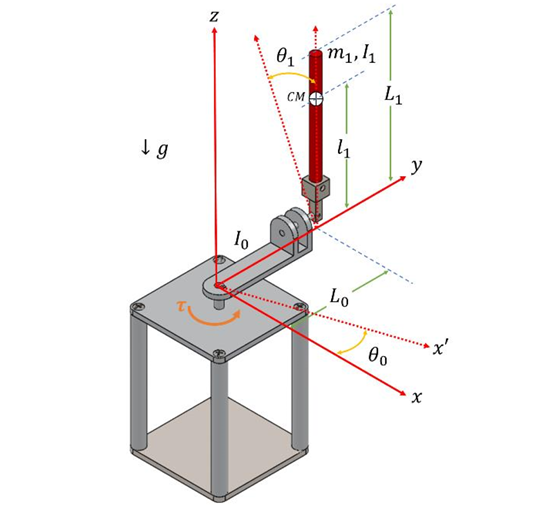
\includegraphics[width=0.85\columnwidth]{figures/pendulo com angulos.png}
        \caption{Representação tridimensional do pêndulo invertido rotacional com seus parâmetros físicos e coordenadas. Fonte: \cite{Duart2017}}
        \label{fig:esquema}
\end{figure} 

\subsection{Objetivo}
O objetivo desta etapa é a obtenção do modelo matemático que descreve a dinâmica do sistema, 
análisar o modelo obtido e simular através do software MATLAB/Simulink.

\section{Modelagem Matemática}
\begin{itemize}
    \item Aplicação das leis da física (Leis de Newton, Lagrange, etc.) para derivar as equações diferenciais que regem o comportamento do sistema.
    \item Linearização do modelo em torno de um ponto de operação, se necessário.
    \item Obtenção da função de transferência $G(s)$ do sistema, relacionando a entrada e a saída.
    \item Apresentação do diagrama de blocos do sistema em malha aberta.
\end{itemize}

\section{Análise do Modelo}

A função de transferência obtida para o sistema foi:
\begin{equation}
    G(s)=\frac{A(s)}{V_m(s)}=\frac{24.59\,s - 0.0024}{s^3 + 14.52s^2 - 81.78s - 637.752}.
\end{equation}

\subsection{Ordem e grau relativo}
\begin{itemize}
    \item \textbf{Ordem do sistema:} 3 (denominador de grau 3) — sistema de 3ª ordem.
    \item \textbf{Grau do numerador:} 1.
\end{itemize}

\subsection{Polos e estabilidade}
As raízes do denominador (polos) obtidos numericamente são aproximadamente:
\[
p_1 \approx -17.12,\qquad p_2 \approx -4.94,\qquad p_3 \approx +7.54.
\]
Como existe um polo em \(\,p_3 \approx +7.54\) (semiplano direito), o sistema é \textbf{instável em malha aberta}. Em termos práticos, qualquer pequena perturbação tenderá a crescer exponencialmente se não houver controle.
A raiz do numerador (zero) é aproximadamente:
\[
z \approx +9.76\times 10^{-5}.
\]
O sistema possui, portanto, um zero no semiplano direito (RHP), caracterizando-o como \textbf{não mínimo-fase}, a principal consequência disso é a tendência do sistema de apresentar uma resposta inversa (undershoot). Se o sistema fosse estável e recebesse um comando em degrau para ir a um valor positivo, a saída primeiro se moveria ligeiramente na direção negativa antes de se corrigir.

No entanto, como o sistema é instável, essa resposta inversa inicial seria rapidamente dominada e mascarada pelo crescimento exponencial causado pelo polo instável.

\subsection{Ganho DC}
O ganho estático do sistema é:
\[
G(0)=\frac{-0.0024}{-637.752}\approx 3.76\times 10^{-6}.
\]
O valor é muito pequeno, mas na prática a dinâmica é dominada pelo polo instável.

\subsection{Tipo do sistema}
Não há polos em $s=0$, logo o sistema é do \textbf{tipo 0}. Em teoria isso significa erro finito para entrada em degrau, mas devido à instabilidade, em malha aberta a saída tende a divergir.

\subsection{Observações finais}
\begin{itemize}
    \item O polo no semiplano direito torna o sistema instável em malha aberta.
    \item O zero no semiplano direito impõe dificuldades na modelagem de um controlador 
\end{itemize}

\section{Simulação Computacional}
\begin{itemize}
    \item Implementação do modelo matemático em software (MATLAB/Simulink ou similar).
    \item Apresentação dos resultados da simulação da resposta do sistema em malha aberta a diferentes sinais de entrada (degrau, impulso).
    \item Discussão e análise crítica dos resultados da simulação.
\end{itemize}

\section{Conclusão Parcial}
\begin{itemize}
    \item Resumo dos resultados obtidos na modelagem e simulação.
    \item Perspectivas para a próxima etapa de montagem e validação.
\end{itemize}

    % \begin{itemize}
    %     \item BREGANON, R. et al. Desenvolvimento de sistemas de pêndulos invertidos como ferramentas didáticas em cursos de engenharia de controle e automação. \textit{HOLOS}, v. 7, p. 1–14, 2021. DOI: 10.15628/holos.2021.10351.
    
    %     \item DUART, J. L. et al. Dynamic modeling and simulation of a rotational inverted pendulum. \textit{Journal of Physics: Conference Series}, v. 792, 2017.
    
    %     \item CASAS, V. M. et al. Construção e projeto de controle de um protótipo de pêndulo invertido rotacional. \textit{EasyChair Preprint}, 2024.
    
    %     \item JAKOBSSON, S. Á. Control of a rotary inverted pendulum system using computer vision. Master’s Thesis – Reykjavik University, 2024.
    
    %     \item YAMANE, L. de S. Projeto mecânico e síntese do controlador de um pêndulo de Furuta. Trabalho de Conclusão de Curso (Engenharia Mecânica) – Universidade Federal do Amazonas, 2020.
    % \end{itemize}


%----------------------------------------------------------
% \nocite{yamane2021}
\printbibliography

%----------------------------------------------------------

\end{document}